\section{30 Oct 2023 - Notes: Deconstructing
Waves}\label{oct-2023---notes-deconstructing-waves}

While we observe waves in many places, it's the case that we don't often
have the luxury of constructing them as we want. In fact, much of the
science we do relies on measurements of voltage or current to represent
the dynamics of the system.

\begin{itemize}
\tightlist
\item
  Want to measure distance? Interferometry gives you a voltage to
  calibrate.
\item
  Want to measure material surface properties? Voltage jumps across
  probes give you proxies
\item
  Viscosity? Stick the stuff in a rheometer, squeeze it, and measure
  voltage changes.
\item
  AYO exoplanets? Light curves are really just measures of voltage
  across a CCD.
\end{itemize}

The point is that you will almost always be dealing with signals that
are proxies for the actual thing you care about. So let's construct some
and deconstruct them.

\subsection{The Cosmic Microwave
Background}\label{the-cosmic-microwave-background}

The
\href{https://en.wikipedia.org/wiki/Cosmic_microwave_background}{Cosmic
Microwave Background} is the oldest light in the universe. It's the
light that was emitted when the universe cooled enough for electrons to
bind to protons and form neutral hydrogen. This happened about 380,000
years after the Big Bang. This signal came in the form of a noise that
was found in every observation we seemed to make. The kind of work we
are starting (signal deconstruction) underlies much of the analysis used
to unpack the CMB, and to continue understanding it. There's a great
video from Fermilab about the CMB.

\href{https://inv.tux.pizza/watch?v=AYFDN2DSVgc}{\pandocbounded{\includegraphics[keepaspectratio,alt={CMB}]{https://markdown-videos-api.jorgenkh.no/youtube/AYFDN2DSVgc?width=720&height=405}}}

\begin{itemize}
\tightlist
\item
  Non-Commercial Link: \url{https://inv.tux.pizza/watch?v=AYFDN2DSVgc}
\item
  Commercial Link: \url{https://youtube.com/watch?v=AYFDN2DSVgc}
\end{itemize}

\subsection{Constructing Waves}\label{constructing-waves}

Below is a little code that will generate superposed waves. We will use
this to generate some intuition about how waves add together, which will
help us deconstruct them.

\begin{Shaded}
\begin{Highlighting}[]
\ImportTok{import}\NormalTok{ numpy }\ImportTok{as}\NormalTok{ np}
\ImportTok{import}\NormalTok{ matplotlib.pyplot }\ImportTok{as}\NormalTok{ plt}
\OperatorTok{\%}\NormalTok{matplotlib inline}

\NormalTok{t }\OperatorTok{=}\NormalTok{ np.linspace(}\DecValTok{0}\NormalTok{,}\DecValTok{2}\NormalTok{,}\DecValTok{1000}\NormalTok{)}
\NormalTok{omega1 }\OperatorTok{=} \DecValTok{100}
\NormalTok{omega2 }\OperatorTok{=} \DecValTok{105}
\NormalTok{omega3 }\OperatorTok{=} \DecValTok{1000}

\NormalTok{A1 }\OperatorTok{=} \DecValTok{1}
\NormalTok{A2 }\OperatorTok{=} \FloatTok{0.9}
\NormalTok{A3 }\OperatorTok{=} \FloatTok{0.1}

\NormalTok{y1 }\OperatorTok{=}\NormalTok{ A1}\OperatorTok{*}\NormalTok{np.cos(omega1}\OperatorTok{*}\NormalTok{t)}

\NormalTok{y2 }\OperatorTok{=}\NormalTok{ A2}\OperatorTok{*}\NormalTok{np.cos(omega2}\OperatorTok{*}\NormalTok{t)}
\NormalTok{y3 }\OperatorTok{=}\NormalTok{ A2}\OperatorTok{*}\NormalTok{np.cos(omega3}\OperatorTok{*}\NormalTok{t)}
\NormalTok{y4 }\OperatorTok{=}\NormalTok{ A3}\OperatorTok{*}\NormalTok{np.cos(omega2}\OperatorTok{*}\NormalTok{t)}
\NormalTok{y5 }\OperatorTok{=}\NormalTok{ A3}\OperatorTok{*}\NormalTok{np.cos(omega3}\OperatorTok{*}\NormalTok{t)}

\NormalTok{CloseAmpCloseFreq }\OperatorTok{=}\NormalTok{ y1}\OperatorTok{+}\NormalTok{y2}
\NormalTok{CloseAmpFarFreq }\OperatorTok{=}\NormalTok{ y1}\OperatorTok{+}\NormalTok{y3}
\NormalTok{FarAmpCloseFreq }\OperatorTok{=}\NormalTok{ y1}\OperatorTok{+}\NormalTok{y4}
\NormalTok{FarAmpFarFreq }\OperatorTok{=}\NormalTok{ y1}\OperatorTok{+}\NormalTok{y5}
\end{Highlighting}
\end{Shaded}

\begin{Shaded}
\begin{Highlighting}[]
\NormalTok{fig }\OperatorTok{=}\NormalTok{ plt.figure(figsize}\OperatorTok{=}\NormalTok{(}\DecValTok{16}\NormalTok{,}\DecValTok{8}\NormalTok{))}


\NormalTok{plt.plot(t,CloseAmpCloseFreq}\OperatorTok{+}\DecValTok{6}\NormalTok{, label}\OperatorTok{=}\StringTok{\textquotesingle{}Close Amp; Close Freq\textquotesingle{}}\NormalTok{)}
\NormalTok{plt.plot(t,CloseAmpFarFreq}\OperatorTok{+}\DecValTok{2}\NormalTok{, label}\OperatorTok{=}\StringTok{\textquotesingle{}Close Amp; Far Freq\textquotesingle{}}\NormalTok{)}
\NormalTok{plt.plot(t,FarAmpCloseFreq}\OperatorTok{{-}}\DecValTok{2}\NormalTok{, label}\OperatorTok{=}\StringTok{\textquotesingle{}Far Amp; Close Freq\textquotesingle{}}\NormalTok{)}
\NormalTok{plt.plot(t,FarAmpFarFreq}\OperatorTok{{-}}\DecValTok{6}\NormalTok{, label}\OperatorTok{=}\StringTok{\textquotesingle{}Far Amp; Far Freq\textquotesingle{}}\NormalTok{)}

\NormalTok{plt.legend()}
\end{Highlighting}
\end{Shaded}

\begin{verbatim}
<matplotlib.legend.Legend at 0x117112f70>
\end{verbatim}

\begin{figure}
\centering
\pandocbounded{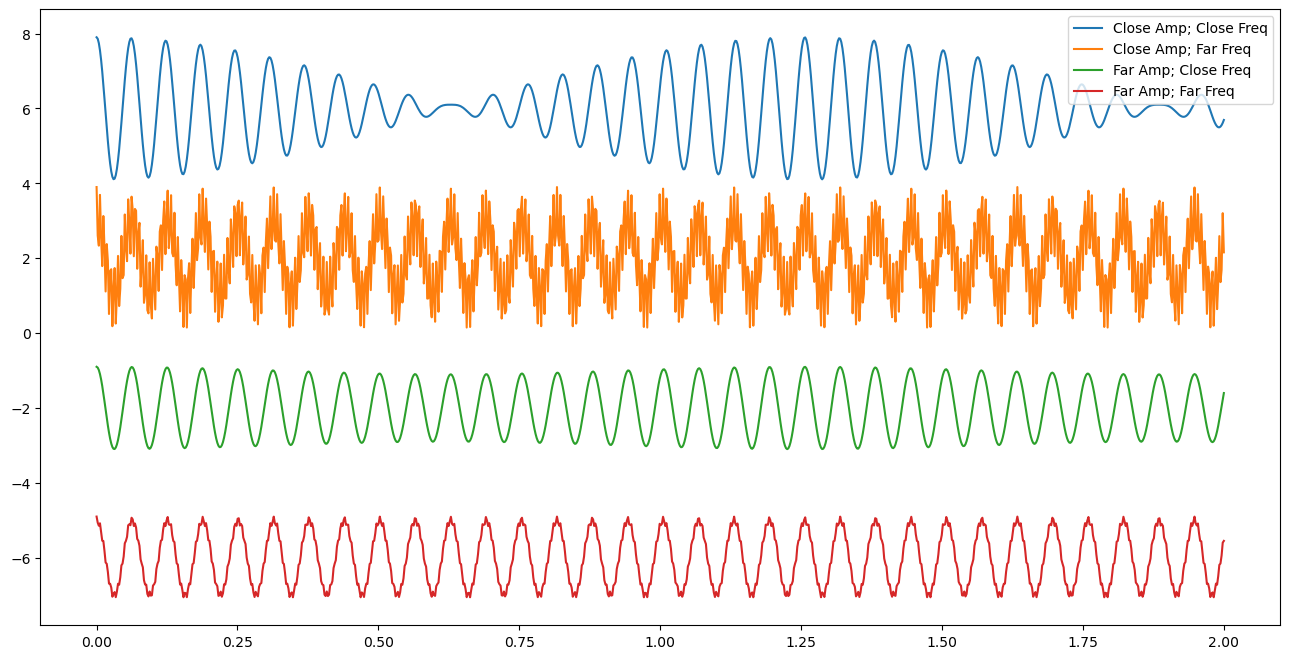
\includegraphics[keepaspectratio,alt={png}]{../images/notes-Waves-Fouriers_Trick_notes-Waves-Fouriers_Trick_tmp_2_1.png}}
\caption{png}
\end{figure}

\textbf{✅ Do this}

\begin{enumerate}
\def\labelenumi{\arabic{enumi}.}
\tightlist
\item
  Adjust the signals to show qualitatively how the different signals
  behave as you change frequencies and amplitudes.
\item
  Build a table that discusses qualitatively what happens as each change
  is made.
\end{enumerate}

Think about the answers to the following questions:

\begin{enumerate}
\def\labelenumi{\arabic{enumi}.}
\tightlist
\item
  Does it seem easier to see how you can deconstruct a superposed wave
  if the frequencies are close together or far apart?
\item
  What about the amplitudes? Does it matter if one is really big and one
  is really small? If they are comparable?
\end{enumerate}

\subsection{Dealing with ``Real''
Signals}\label{dealing-with-real-signals}

Ok, but can we find these frequencies given a signal? Or rather, how
might we find the signal we need? We can use a little mathematics from
Fourier. The
\href{https://en.wikipedia.org/wiki/Fourier_transform}{Fourier
transform} is a mathematical tool that allows us to deconstruct a signal
into its constituent frequencies. There's an excellent introduction to
it from 3Blue1Brown.

\href{https://inv.tux.pizza/watch?v=spUNpyF58BY}{\pandocbounded{\includegraphics[keepaspectratio,alt={Fourier Transform}]{https://markdown-videos-api.jorgenkh.no/youtube/spUNpyF58BY?width=720&height=405}}}

\begin{itemize}
\tightlist
\item
  Non-Commercial Link: \url{https://inv.tux.pizza/watch?v=spUNpyF58BY}
\item
  Commercial Link: \url{https://youtube.com/watch?v=spUNpyF58BY}
\end{itemize}

So any periodic function in 1 dimension can be expanded as a general sum
of sines and cosines:

\[f(t) = \dfrac{a_0}{2} + \sum_{n=1}^{\infty} \left(a_n sin(\omega_n t) + b_n cos(\omega_n t) \right)\]

We can show this can be written like:

\[f(t) = \sum_{-\infty}^{+\infty} c_n e^{i\omega_n t}\]

But how does this get us what we need? Our goal is to find the expansion
coefficients (\(a_n\)'s \& \(b_n\)'s or just the \(c_n\)'s), which tells
us the right mix of signals to add together to get the observed one. Why
is that important? Consider the signals below? How might we analyze
them?

\begin{Shaded}
\begin{Highlighting}[]
\ImportTok{from}\NormalTok{ scipy.signal }\ImportTok{import}\NormalTok{ sawtooth, square, chirp}

\NormalTok{t }\OperatorTok{=}\NormalTok{ np.linspace(}\DecValTok{0}\NormalTok{,}\DecValTok{10}\NormalTok{,}\DecValTok{1000}\NormalTok{)}

\NormalTok{saw }\OperatorTok{=}\NormalTok{ sawtooth(t)}
\NormalTok{sq }\OperatorTok{=}\NormalTok{ square(t)}
\NormalTok{ch }\OperatorTok{=}\NormalTok{ chirp(t,}\DecValTok{6}\NormalTok{,}\DecValTok{10}\NormalTok{,}\DecValTok{1}\NormalTok{)}

\NormalTok{fig }\OperatorTok{=}\NormalTok{ plt.figure(figsize}\OperatorTok{=}\NormalTok{(}\DecValTok{12}\NormalTok{,}\DecValTok{8}\NormalTok{))}
\NormalTok{plt.plot(t, saw, label}\OperatorTok{=}\StringTok{"Sawtooth Wave"}\NormalTok{)}
\NormalTok{plt.plot(t, sq}\OperatorTok{+}\DecValTok{3}\NormalTok{, label}\OperatorTok{=}\StringTok{\textquotesingle{}Square Wave\textquotesingle{}}\NormalTok{)}
\NormalTok{plt.plot(t, ch}\OperatorTok{{-}}\DecValTok{3}\NormalTok{, label}\OperatorTok{=}\StringTok{\textquotesingle{}Chirp\textquotesingle{}}\NormalTok{)}
\NormalTok{plt.legend()}
\end{Highlighting}
\end{Shaded}

\begin{verbatim}
<matplotlib.legend.Legend at 0x17b39f670>
\end{verbatim}

\begin{figure}
\centering
\pandocbounded{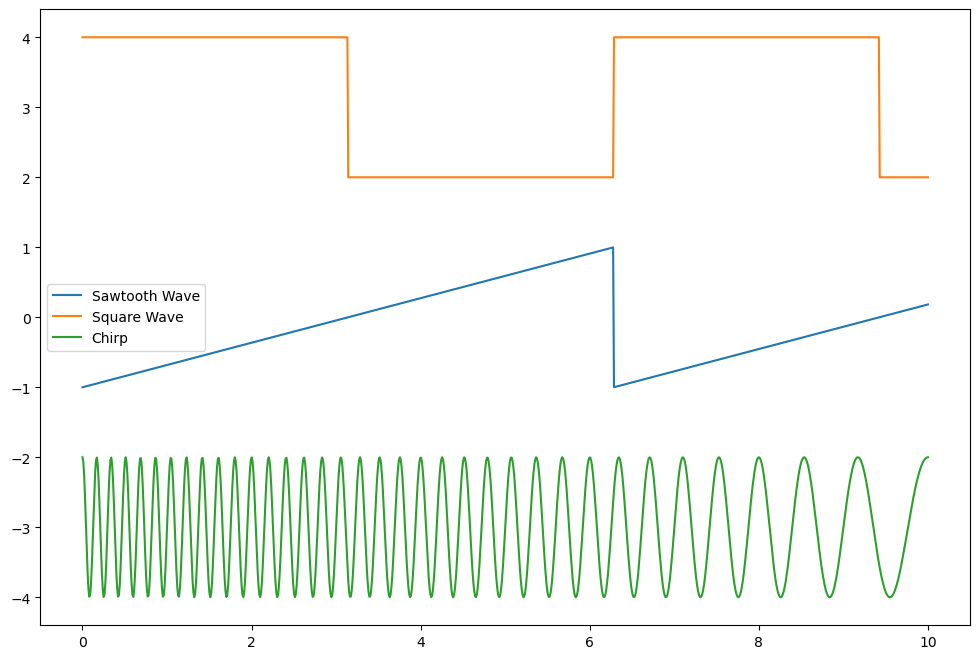
\includegraphics[keepaspectratio,alt={png}]{../images/notes-Waves-Fouriers_Trick_notes-Waves-Fouriers_Trick_tmp_5_1.png}}
\caption{png}
\end{figure}

\subsection{Decomposing Signals}\label{decomposing-signals}

Consider the Fourier Expansion of your choosing:

\[f(t) = \dfrac{a_0}{2} + \sum_{n=1}^{\infty} \left(a_n \sin(\omega_n t) + b_n \cos(\omega_n t) \right) \qquad f(t) = \sum_{-\infty}^{+\infty} c_n e^{i\omega_n t}\]

In terms of the longest period, \(T_0\),

\[f(t) = \dfrac{a_0}{2} + \sum_{n=1}^{\infty} \left(a_n \sin(\dfrac{2n\pi t}{T_0}) + b_n \cos(\dfrac{2n\pi t}{T_0}) \right) \qquad f(t) = \sum_{-\infty}^{+\infty} c_n e^{i\dfrac{2n\pi t}{T_0}}\]

We can find the expansion coefficients for the following signals (think
before you integrate):

\begin{enumerate}
\def\labelenumi{\arabic{enumi}.}
\tightlist
\item
  \(f(t) = \cos(\omega_0 t)\) here \(\omega_0\) corresponds to the
  longest known period \(T_0\).
\item
  \(f(t) = 2\sin(\omega_0 t) + 3\cos(2*\omega_0t)\)
\item
  \(f(t) = 2\sin(\omega_0 t+\pi/2) + 3\cos(2*\omega_0t)\)
\item
  \(f(t) = 1\) from 0 to \(T_0/2\) and 0 from \(T_0/2\) to \(T_0\)
  repeating\ldots.
\end{enumerate}

\subsubsection{Pick off the
coefficients}\label{pick-off-the-coefficients}

For the first two cases, we can pick off the coefficients because they
match the model

\[f(t) = \dfrac{a_0}{2} + \sum_{n=1}^{\infty} \left(a_n \sin(\dfrac{2n\pi t}{T_0}) + b_n \cos(\dfrac{2n\pi t}{T_0}) \right)\]

For \(f(t) = \cos(\omega_0 t)\), all the terms are zero except for
\(b_1\) which is 1.

For \(f(t) = 2 \sin(\omega_0 t) + 3 \cos(2\omega_0 t)\), all the terms
are zero except for \(a_1\) which is 2 and \(b_2\) which is 3.

What about the 3rd one?

\[f(t) = 2\sin(\omega_0 t+\pi/2) + 3\cos(2*\omega_0t)\]

It's clever to change this to a cosine and read off the values:

\[f(t) = 2\sin(\omega_0 t+\pi/2) + 3\cos(2*\omega_0t) = 2\cos(\omega_0 t) + 3\cos(2*\omega_0t)\]

And thus: \(b_1 = 2\) and \(b_2=3\) and everything else vanishes.

Can we do the integrals and get the same results? Sure. But it's a lot
more work.

\subsubsection{What about the last one?}\label{what-about-the-last-one}

That function is a classic ``square wave'', or
\href{https://en.wikipedia.org/wiki/Duty_cycle}{half duty cycle}. It's a
function that is 1 for half the period and 0 for the other half. It's a
function that is used in digital electronics to encode information. That
function we have to solve by integrating. The handwritten notes show
how. The more general duty cycle function is shown below.

\begin{figure}
\centering
\pandocbounded{\includegraphics[keepaspectratio,alt={Duty cycle gif}]{https://upload.wikimedia.org/wikipedia/commons/0/02/PWM_duty_cycle_with_label.gif}}
\caption{Duty cycle gif}
\end{figure}

\subsection{Resources}\label{resources}

\subsubsection{Handwritten notes}\label{handwritten-notes}

\begin{itemize}
\tightlist
\item
  \href{../assets/notes/Notes-Fourier_Example.pdf}{Introduction to
  Signal Analysis}
\end{itemize}

\subsubsection{Additional Videos}\label{additional-videos}

\href{https://inv.tux.pizza/watch?v=mgXSevZmjPc}{\pandocbounded{\includegraphics[keepaspectratio,alt={Fourier Series}]{https://markdown-videos-api.jorgenkh.no/youtube/mgXSevZmjPc?width=720&height=405}}}

\begin{itemize}
\tightlist
\item
  Non-Commercial Link: \url{https://inv.tux.pizza/watch?v=mgXSevZmjPc}
\item
  Commercial Link: \url{https://youtube.com/watch?v=mgXSevZmjPc}
\end{itemize}
